\section{Proposed Approach}
\label{sec:approach}
%NetML takes as input a new bug report as well as a \emph{historical} set of previously localized bug cases, each comprising a bug report and a set of (faulty) methods along with their program spectra. If a method contains a root cause of the bug, it is labeled as \textit{faulty} or \textit{relevant}, otherwise it is labeled as \textit{non-faulty} or \textit{irrelevant}. 

An overview of our NetML framework is given in Figure~\ref{fig:framework} (enclosed in the dashed box). 
NetML takes as input a new bug report, the program spectra corresponding to it, and a method corpus. It also takes as input \emph{historical} bug reports that have been localized before. For each \textit{historical} bug report, we have its corresponding program spectra and ground truth labels. If a method contains a root cause of the bug, it is labeled as \textit{faulty}, otherwise it is labeled as \textit{non-faulty}. Given these inputs, NetML eventually produces a list of methods, ranked based on their likelihood to contain the root cause of the new bug report.

%, and outputs a list of methods ranked based on their likelihood to be faulty. To produce its output, NetML also analyzes \emph{historical} bug reports, their corresponding program spectra as well as a method corpus. 
%If a method contains a root cause of the bug, it is labeled as \textit{faulty} or \textit{relevant}, otherwise it is labeled as \textit{non-faulty} or \textit{irrelevant}. Given a new bug report and its corresponding program spectra, NetML looks at the historical set of previously localized bugs, their corresponding spectra, as well as the relevant method corpus, and then produces 
%Given a new bug report, NetML looks at the historical set of previously localized bugs as well as the relevant method corpus and program spectra, and then produces a list of methods ranked based on their likelihood to be faulty. %The approach can also be generalized to localize bugs at other levels of granularity, especially coarser levels of granularity, e.g., files or basic blocks or statements.

NetML has three main components, namely: \emph{feature extraction}, \emph{graph construction}, and \emph{integrator}. The feature extraction component serves to extract multi-modal input features that quantify different perspectives on the degree of relevancy between a bug report and a method. Note that this is in a similar spirit to~\cite{Le:2015:IRS:2786805.2786880}. Meanwhile, the graph construction component computes the similarity graphs among the bug reports ($\mathcal{G}_B$) and methods ($\mathcal{G}_M$).

Finally, the integrator component is the heart of NetML and constitutes the primary contribution of this work. It integrates both input features and similarity graph information in order to produce a ranked list of methods based on their relevancy score. In particular, the integrator performs adaptive learning that aims at jointly minimizing the bug localization errors and fostering clustering of the latent parameters of similar bug reports and/or methods.

In Sections \ref{sec.generalized_adaptive}--\ref{sec:learning}, we first describe the NetML integrator component in greater details, including the formulation of our new integrator model as well as the corresponding objective function and adaptive learning procedure. We then elaborate the feature extraction and graph construction components in Sections \ref{subsec:feature} and \ref{subsec:graph}, respectively.

%Similar to AML~\cite{Le:2015:IRS:2786805.2786880}, NetML also has four components: $\text{NetML}^\text{Text}_{b,m}$, $\text{NetML}^\text{Spectra}_{m}$, NetML$^\text{SuspWord}$, and NetML$^\text{Integrator}$. $\text{NetML}^\text{Text}_{b,m}$ processes only the textual information in the input bug reports using an IR-based bug localization technique described in Section~\ref{sec.prelim}. $\text{NetML}^\text{Text}_{b,m}$ in the end outputs a score for each method in the corpus. Given a bug report $b$ and a method $m$ in a corpus $C$, $\text{NetML}^\text{Text}_{b,m}$ outputs a score that indicates how close is $m$ to $b$ which is denoted as NetML$^\text{Text}(b,m,C)$. By default, $\text{NetML}^\text{Text}_{b,m}$ uses VSM as the IR-based bug localization technique.

\begin{figure}[!t]
\centering
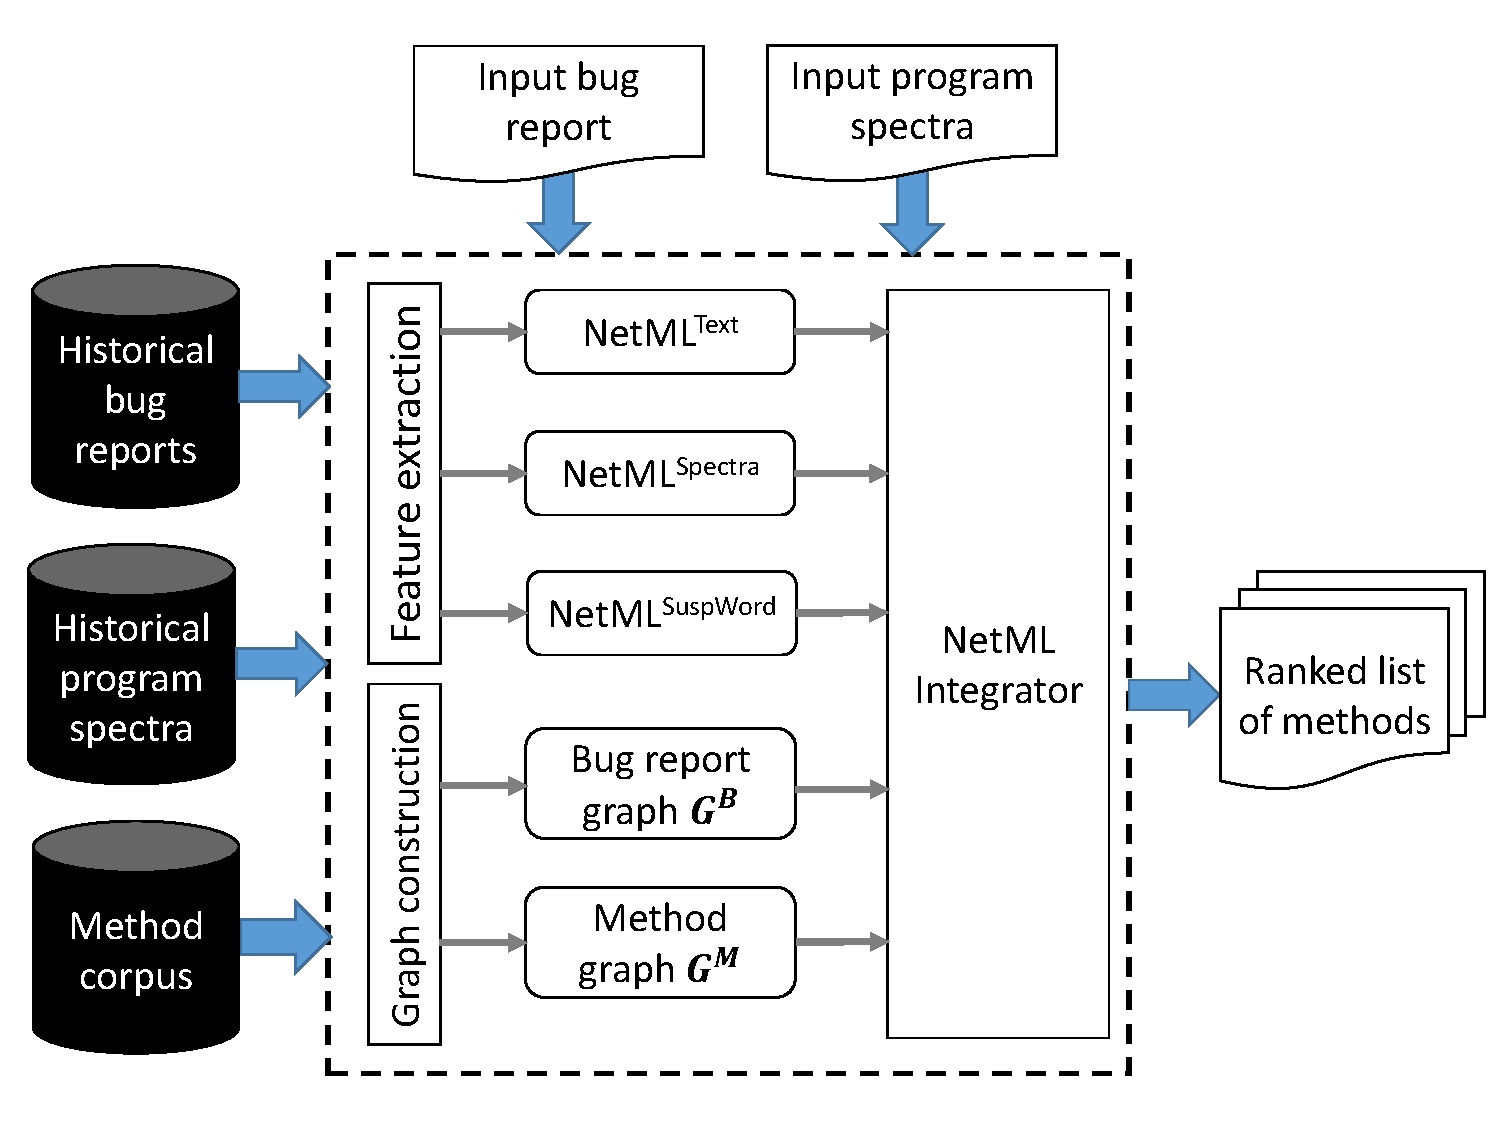
\includegraphics[width=0.5\textwidth]{netml_framework}
\caption{The proposed NetML framework}
\label{fig:framework}
\end{figure}

\subsection{Feature Extraction}
\label{subsec:feature}


The second component of the NetML framework is the feature extraction module, which generates features $\mathbf{X} = \{ x_{b,m.j} \}$ to be fed as inputs to the NetML integrator (see  Fig. \ref{fig:framework}). In line with our earlier AML work \cite{Le:2015:IRS:2786805.2786880}, for each bug report--method pair $(b,m)$, we compute a feature vector $\vec{x}_{b,m}$  that consists of three elements (i.e., $J = 3$):
\begin{align}
\vec{x}_{b,m} = \left[ \text{NetML}^\text{Text}_{b,m}, \text{NetML}^\text{Spectra}_{b, m}, \text{NetML}^\text{SuspWord}_{b,m} \right]
\end{align}
The three features are elaborated in turn below.



$\text{NetML}^\text{Text}_{b,m}$ makes use of the TF-IDF method~\cite{Ramos1999} to estimate the similarity between methods and bug reports. In particular, given a method $m$ and a bug report $b$, $\text{NetML}^\text{Text}_{b,m}$ computes the cosine similarity between the TF-IDF representation of the bug report text and that of the method codes, which is akin to the IR-based bug localization method (cf. Section~\ref{sec.IR-based}). That is, $\text{NetML}^\text{Text}_{b,m}$ is given by:
\begin{align}
\text{NetML}^\text{Text}_{b,m} = sim(b,m)	
\end{align}
where $sim(b,m)$ is the cosine similarity as defined in (\ref{eqn:cosine_sim}).


$\text{NetML}^\text{Spectra}_{b, m}$ processes only the program spectra information using a spectrum-based bug localization technique described in Section~\ref{sec.spectrum-based}. Given a program spectra $p$ corresponding to bug report $b$ and a method $m$, $\text{NetML}^\text{Spectra}_{b, m}$ gives a score that quantifies how suspicious  $m$ is given $p$. By default, $\text{NetML}^\text{Spectra}_{b, m}$ uses the Tarantula method as described in Section \ref{sec.spectrum-based} (cf. equation (\ref{eqn:tarantula})):
\begin{align}
\text{NetML}^\text{Spectra}_{b, m} = Tarantula(m, p)
\end{align}


Finally, $\text{NetML}^\text{SuspWord}_{b,m}$ processes both bug reports and program spectra, and computes the suspiciousness scores of words to rank different methods. It breaks a method into its constituent words, computes the suspiciousness scores of these words, and then aggregates these scores back in order to arrive at the suspiciousness score of the method. Given a bug report $b$, a program spectra $p$, and a method $m$ in a corpus $C$, $\text{NetML}^\text{SuspWord}_{b,m}$ measures how suspicious $m$ is considering $b$ and $p$,  as follows: %Thus, NetML$^\text{SuspWord}$ involves three basic steps: mapping of methods to words, computing word suspiciousness, and composing word suspiciousness into method suspiciousness. 
\begin{align}
&\text{NetML}^\text{SuspWord}_{b,m} = \text{NetML}^\text{Spectra}_{b, m} \times \\
%\text{SS}_{\text{method}}(m,p)\nonumber \times\\
&\frac{\sum\limits_{w\in b \cap m} \text{SSTFIDF}(w,p,b,C)\times \text{SSTFIDF}(w,p,m,C)}{\sqrt{\sum\limits_{w \in b} \text{SSTFIDF}(w,p,b,C)^2} \times \sqrt{\sum\limits_{w \in m} \text{SSTFIDF}(w,p,m,C)^2}}
\label{eq:sum_vsm_susp}
\end{align}
where 
%$\text{SS}_{\text{method}}(m,p)$ is the suspiciousness scores of a method, which by default uses  the same score as the NetML$^{spectra}(m)$ component, and 
$\text{SSTFIDF}(w,p,b,C)$ is the weight of a word $w$ in document (i.e., bug report or method) $d$ with corpus $C$ given program spectra $p$:
\begin{align}
\text{SSTFIDF}(w,p,d,C) = &\text{SS}_{\text{word}}(w,p)\times \ln(f(w,d)+1) \nonumber\\
&\times \ln\frac{|C|}{|{d_i\in C : w \in d_i }|}
\end{align}
where $\text{SS}_{\text{word}}(w,p)$ is the suspiciousness score of a word $w$:
\begin{align}
\text{SS}_{\text{word}}(w,p) &= \frac{\frac{|EF(w,p)|}{|p.FAIL|}}{\frac{|EF(w,p)|}{|p.FAIL|}+\frac{|ES(w,p)|}{|p.SUCCESS|}}
\label{eq:ss}
\end{align}
In the above equation, $EF(w,p)$ is the set of execution traces in $p.FAIL$ that contain a method in which the word $w$ appears, while $ES(w,p)$ is the set of execution traces in $p.SUCCESS$ that contain a method in which the word $w$ appears. Further details of all these components can be found in~\cite{Le:2015:IRS:2786805.2786880}.


%\recheck{Altogether, the three features that provide a multi-modal perspective on the degree of relevancy between a bug report and a method, are then sent to the NetML integrator in order to produce a ranked list of methods (given a bug report $b$ (cf. Fig.~\ref{fig:framework}).}

%The $\text{NetML}^\text{Text}_{b,m}$ and $\text{NetML}^\text{Spectra}_{m}$  components reuse techniques proposed in prior works which are described in Section~\ref{sec.prelim}. In the next subsections, we briefly describe the components namely NetML$^\text{SuspWord}$ and the network-clustered integrator component.
%
%Parnin and Orso {highlighted} that ``future research could also investigate ways to automatically suggest or highlight terms that might be related to a failure''~\cite{ParninO11}, however they did not propose a concrete solution. We use Parnin and Orso's observation, which highlights that some words are indicative to the location of a bug, as a starting point to design our NetML$^\text{SuspWord}$ component. \iffalse NetML$^\text{SuspWord}$ component is designed based on this observation made by Parnin and Orso which highlights that some words are indicative to the location of a bug.\fi
%This component breaks down a method into its constituent words, computes the suspiciousness scores of these words, and composes these scores back to result in the suspiciousness score of the method. The process is analogous to a machine learning or classification algorithm that breaks a data point into its constituent features, assign weights or importance to these features, and use these features, especially important ones, to assign likelihood scores to the data point. The component works in three steps: mapping of methods to words, computing word suspiciousness, and composing word suspiciousness into method suspiciousness. We describe each of these steps in the following sections. 
%
%% component takes in a spectra and a bug report to compute the suspiciousness scores of words. The suspicious words are then used to rank methods. Different from the $AML^{SPECTRA}$ component that directly computes the suspiciousness scores of methods, this
%
%\subsubsection{Mapping of Methods to Words}
%In this step, we map a method to its constituent words. For every method, we extract the following textual contents including: (1) The name of the method, along with the names of its parameters, and identifiers contained in the method body; (2) The name of the class containing the method, and the package containing the class; (3) The comments that are associated to the method (e.g., the Javadoc comment of that method, and the comments that appear inside the method), and comments that appear in the class (containing the method) that are not associated to any particular method.
%
%After we have extracted the above textual contents, we apply the text pre-processing step described in Section~\ref{sec.prelim}. At the end of this step, for every method we map it to a set of pre-processed words. Given a method $m$, we denote the set of words it contains as $words(m)$.
%
%\subsubsection{Computing Word Suspiciousness}
%We compute the suspiciousness score of a word by considering the program elements that contain the word. Let us denote the set of all failing execution traces in spectra $p$ as $p.F$ and the set of all successful execution traces as $p.S$. To compute the suspiciousness scores of a word $w$ given spectra $p$, we define several sets:
%%\begin{eqnarray}
%%EF(w,p) = \{t \in p.F | \exists {m\in t}~s.t.~w\in words(m)\}\footnotemark[1]\nonumber\\
%%NF(w,p) = \{t \in p.F | \not\exists {m\in t}~s.t.~w\in words(m)\}\nonumber\\
%%ES(w,p) = \{t \in p.S | \exists {m\in t}~s.t.~w\in words(m)\}\nonumber\\
%%NS(w,p) = \{t \in p.S | \not\exists {m\in t}~s.t.~w\in words(m)\}\nonumber
%%\end{eqnarray}
%\begin{align*}
%EF(w,p) &= \{t \in p.F | \exists {m\in t}~s.t.~w\in words(m)\}\nonumber\\
%%NF(w,p) &= \{t \in p.F | \not\exists {m\in t}~s.t.~w\in words(m)\}\nonumber\\
%ES(w,p) &= \{t \in p.S | \exists {m\in t}~s.t.~w\in words(m)\}\nonumber
%%NS(w,p) &= \{t \in p.S | \not\exists {m\in t}~s.t.~w\in words(m)\}\nonumber
%\end{align*}
%The set $EF(w,p)$ is the set of execution traces in $p.F$ that contain a method in which the word $w$ appears. The set $ES(w,p)$ is the set of execution traces in $p.S$ that contain a method in which the word $w$ appears. Based on these sets, we can compute the suspiciousness score of a word $w$ using a formula similar to Tarantula as follows:
%\begin{equation}
%\text{SS}_{\text{word}}(w,p)=\frac{\frac{|EF(w,p)|}{|p.FAIL|}}{\frac{|EF(w,p)|}{|p.FAIL|}+\frac{|ES(w,p)|}{|p.SUCCESS|}}
%\label{eq:ss}
%\end{equation}
%
%Using the above formula, words that appear more often in methods that are executed in failing execution traces are deemed to be more suspicious than those that appear less often in such methods.
%
%%The set $NF(w,p)$ is the set of execution traces in $p.F$ that do not contain a method in which the word $w$ appears. The set $NS(w,p)$ is the set of execution traces in $p.S$ that do not contain a method in which the word $w$ appears.
%
%\subsubsection{Computing Method Suspiciousness}
%To compute a method $m$'s suspiciousness score, we compute the textual similarity between $m$ and the input bug report $b$, and consider the appearances of $m$ in the input program spectra $p$. In the textual similarity computation, the suspiciousness of words are used to determine their weights.
%
%First, we create a vector of weights that represents a bug report and another vector of weights that represents a method. Each element in a vector corresponds to a word that appears in either the bug report or the method. The weight of a word $w$ in document (i.e., bug report or method) $d$ of method corpus $C$ considering program spectra $p$ is:
%\begin{align*}
%\text{SSTFIDF}(w,p,d,C)=&\text{SS}_{\text{word}}(w,p)\times \ln(f(w,d)+1)\\
%&\times \ln\frac{|C|}{|{d_i\in C : w \in d_i }|}
%\end{align*}
%In the above formula, $\text{SS}_\text{word}(w,p)$ is the suspiciousness score of word $w$ computed by Equation~\ref{eq:ss}, $f(w,d)$ is the number of times word $w$ appears in document $d$, and $d_i \in C$ means document $d_i$ is in the set of document $C$. Similarly, $w \in d_i$ means word $w$ belongs to document $d_i$. The above formula considers the weight of a word based on its suspiciousness, and well-known information retrieval metrics: term frequency (i.e., $\ln(f(w,d)+1)$) and inverse document frequency (i.e., $\ln\frac{|C|}{|{d_i\in C : w \in d_i }|}$).
%
%After the two vectors of weights of method $m$ and bug report $b$ are computed, we compute the suspiciousness score of the method $m$ by computing the cosine similarity of these two vectors multiplied by a weighting factor. The formula to compute this score is as follows:
%\begin{align}
%&\text{AML}^\text{SuspWord}(b,p,m,C)=\text{SS}_{\text{method}}(m,p)\nonumber \times\\
%&\frac{\sum\limits_{w\in b \cap m} \text{SSTFIDF}(w,p,b,C)\times \text{SSTFIDF}(w,p,m,C)}{\sqrt{\sum\limits_{w \in b} \text{SSTFIDF}(w,p,b,C)^2} \times \sqrt{\sum\limits_{w \in m} \text{SSTFIDF}(w,p,m,C)^2}}
%\label{eq:sum_vsm_susp}
%\end{align}
%Here we use $\text{SS}_\text{method}(m,p)$ that computes the suspiciousness score of method $m$ considering program spectra $p$ as the weighting factor. This can be computed by various spectrum-based bug localization tools. By default, we use the same fault localization tool as the one used in $\text{NetML}^\text{Spectra}_{m}$ component. With this, NetML$^\text{SuspWord}$ integrates both macro view of method suspiciousness (which considers direct execution of a method in the failing and correct execution traces) and micro view of method suspiciousness (which considers the executions of its constituent words in the execution traces).

\subsection{Graph Construction}
\label{subsec:graph}

The final component of the NetML framework is the graph construction module, which serves to compute the similarity graphs among bug reports and methods, to be used in the K-nearest neighbor retrieval as well as the network Lasso regularization. In this work, we define the bug report similarity graph $\mathcal{G}_B$ as comprising edge weights that reflect the textual similarity between two bug reports. For a pair of bug reports $b$ and $b'$, we define the edge weight $e_{b.b'}$ as:
\begin{align}
\label{eqn:edge_b}
e_{b,b'} = sim(b, b')
\end{align}
where $sim(b,b')$ is the cosine similarity between the TF-IDF weights of the textual descriptions of $b$ and $b'$, as per (\ref{eqn:cosine_sim}).


Similarly, the method similarity graph $\mathcal{G}_M$ comprises a set of edge weights $e_{m,m'}$ that reflect the textual similarity between two methods $m$ and $m'$. This is given by:
\begin{align}
\label{eqn:edge_m}
e_{m,m'} = sim(m, m')
\end{align}
where $sim(b,b')$ is the cosine similarity between the TF-IDF representations of the source codes of $m$ and $m'$.


\subsection{Integrator Model}
\label{sec.generalized_adaptive}

%As we mention in Section~\ref{sec.intro}, \underline{A}daptive \underline{M}ulti-modal bug \underline{L}ocalization (AML)~\cite{Le:2015:IRS:2786805.2786880} remains two main issues. Firstly, AML only proposes the concept of latent parameter for bug reports. In particular, every method $m$ share the same bug report parameter when estimating the suspiciousness scores of $m$, without considering the method parameter. Hence, AML may not capture the properties of different methods, leading to limit its effectiveness of detecting bug. Secondly, the latent paprameter of each bug report is learned independently of other bug report, without exploiting the clustering and/or similarity properties of different bug reports and methods. In practice, some bug reports as well as methods are similar to other bug reports/methods. However, AML simply ignores the relationship between bug reports and methods. 

The new integrator model proposed in this work characterizes the relevancy of a method $m$ to a given bug report $b$ as an interaction between two types of latent parameters, namely: \emph{latent bug report parameters} $\vec{u}_b = [u_{b,1}, \ldots, u_{b,j}, \ldots, u_{b,J}]$ and \emph{latent method parameters} $\vec{v}_m = [v_{m,1}, \ldots, v_{m,j}, \ldots, v_{m,J}]$, where $J$ is the total number of features. More specifically, the integrator model computes the relevancy score $\hat{f}_{b,m}$ as follows: 
%The first is to redefine the suspiciousness score of method $m$ given by bug reports $b$ as an interaction between a bug report’s parameter vector $\vec{u}_b$ and a method’s parameter vector $\vec{v}_m$. In particular, NetML 
%We propose \underline{N}etwork-clustered \underline{M}ulti-modal Bug \underline{L}ocalization (NetML) that involves two extensions. The first is to redefine the suspiciousness score of method $m$ given by bug reports $b$ as an interaction between a bug report’s parameter vector $\vec{u}_b$ and a method’s parameter vector $\vec{v}_m$, as follows: 
%The first is to redefine the function of suspiciousness score (see equation \ref{eqn:composite}) as an interaction between a bug report’s parameter vector $\vec{u}_b$ and a method’s parameter vector $\vec{v}_m$, as follows:
\begin{align}
\label{eq:aml_plus}
\hat{f}_{b,m} = \hat{f}(\vec{x}_{b,m}, \vec{u}_b, \vec{v}_m) = \sum_{j = 1}^{J} (u_{b,j} + v_{m,j}) x_{b,m,j}
\end{align}
where $\vec{x}_{b,m} = [x_{b,m,1}, \ldots, x_{b,m,j}, \ldots, x_{b,m,J}]$ is the feature vector corresponding to a bug report--method pair $(b, m)$.

It is worth mentioning that the above model constitutes a generalization of the AML integrator model that we previously developed~\cite{Le:2015:IRS:2786805.2786880}. In AML, the final relevancy score is computed based solely on the latent bug report parameters, and this set of parameters is shared by all methods for a given bug report. On the other hand, the NetML integrator model accounts for not only the latent bug report parameters but also the latent method parameters. The addition of the latter parameters provides a greater degree of freedom/flexibility in quantifying the contribution of different methods to the localization of a given bug report.

%In light of these issues, we propose a new algorithm, namely \underline{N}etwork-clustered \underline{M}ulti-modal Bug \underline{L}ocalization (NetML). More specifically, NetML tries to addresses these two shortcomings by performing joint optimization of localization loss function and clustering of both bug reports and methods. Firstly, NetML integrates two sets of latent parameters (i.e., bug reports and methods) to localize bug more accurately. Secondly, NetML takes advantage of network Lasso regularization~\cite{Hallac:2015:NLC:2783258.2783313} to enforce similar bug reports as well as methods to have similar latent parameters. Thus, the proposed approaches may achieve a more effective bug localization. 
%
%In the following section, we firstly present a short introduction about network Lasso, and briefly explain our proposed algorithm, i.e., NetML. 
%
%
%%Firstly, for each bug report $b$, a fixed parameter vector $\vec{\theta}_b = (\alpha, \beta, \gamma)$ is inferred for all methods $m$ (see Equation~\ref{eqn:composite}). 
%%In other words, every method $m$ shares the same parameter vector $\vec{\theta}_b$ when estimating the suspiciousness scores of $m$ according to bug report $b$ and program spectra $p$. In particular, each method $m$ not only considers the parameter of bug report $b$ but also share the parameter of method $m$. 
%%Therefore, Equation~\ref{eqn:composite} does not accurately reflect the suspiciousness score of method $m$ given bug report $b$ and program spectra $p$. Secondly, the parameter vector $\vec{\theta}_b$ of a bug report is learned independently of other bug report $b'$, without exploiting the clustering and/or similarity properties of different bug reports and methods. In practice, some bug reports as well as methods are similar to other bug reports/methods. However, the instance-wise loss function in equation \ref{eq:instance-wise-loss} ignores the relationship between the bug reports and the methods. In light of these issues, we proposed a new algorithm, namely generalized adaptive multi-modal bug localization, to tackle these problems in bug localization. 
%
%%Our proposed algorithm is inspired by network lasso \cite{Hallac:2015:NLC:2783258.2783313}. In the next sub section, I briefly present a short introduction about network lasso, then explain the proposed algorithm, i.e. \underline{G}eneralized \underline{A}daptive \underline{M}ulti-modal bug \underline{L}ocalization (AML*).
%
%\subsubsection{Network Lasso}\label{subsec:networklasso}
%
%Nowadays, convex optimization has become a popular way of modeling problems in many different fields (i.e., clock synchronization, smart power grids, state estimation, etc.). However, classical methods of convex analysis, relying on interior point methods~\cite{Renegar:2001:MVI:502968}, begin to fail due to a lack of scalability since datasets is getting larger and more intricate. The challenge of large-scale optimization lies in developing methods general enough to work well independent of the input, while being capable of scaling to the immense datasets that today’s applications require. In~\cite{Hallac:2015:NLC:2783258.2783313}, Hallac et al. proposed a network setting, namely network Lasso, that allows for simultaneous clustering and optimization on graph. In particular, given a graph $\mathcal{G}=(\mathcal{V}, \mathcal{E})$, where $\mathcal{V}$ is the vertex set and $\mathcal{E}$ is the edges of graph. The network Lasso problem is defined as following: 
%
%%Therefore, it is necessary to formulate general classes of convex optimization solvers, ones that can apply to a variety of interesting and relevant problems, and to develop algorithms for reliable and efficient solutions.
%
%%Network Lasso~\cite{Hallac:2015:NLC:2783258.2783313} is a generalization of the group lasso to a network setting that allows for simultaneous clustering and optimization on graphs. In~\cite{Hallac:2015:NLC:2783258.2783313}, Hallac et al. focused on optimization problem posed on graph. Given a graph $\mathcal{G}=(\mathcal{V}, \mathcal{E})$, where $\mathcal{V}$ is the vertex set and $\mathcal{E}$ is the edges of graph. The network lasso problem is defined as following: 
%\begin{align}
%\label{eq:network_lasso}
%	minimize \sum_{i \in \mathcal{V}}^{} f_i(\vec{x}_{b,m}) + \lambda \sum_{(j, k) \in \mathcal{E}}^{} w_{jk} \|x_j - x_k \|_{2}	
%\end{align}
%The variable are $x_1, \dots, x_n \in R^{p}$, where $n = |\mathcal{V}|$. $\vec{x}_{b,m} \in R^{p}$ is the variable at node $i$, $f_i$ is the cost function at node $i$, $w_{jk}$ is the relative weights among the edges $(j,k)$ of the network $\mathcal{G}$, and $\lambda$ is an overall parameter that scales the edge objectives relative to the node objectives. In order to solve the problem \ref{eq:network_lasso} in a distributed and scalable manner, which allows for guaranteed global convergence even on large graphs, the author based on the Alternating Direction Method of Multipliers (ADMM)~\cite{Parikh:2014:PA:2693612.2693613, Boyd:2011:DOS:2185815.2185816}. With ADMM, each individual component solves its own private objective function, passes this solution to its neighbors, and repeats the process until the entire network converges. 

\subsection{Objective Function}
\label{subsec:objective}

%The second extension takes advantage of network Lasso regularization~\cite{Hallac:2015:NLC:2783258.2783313} to enforce similar bug reports as well as methods to have similar latent parameters. Different from the original network Lasso that only deals with a single graph, our approach involves optimizing over two graphs simultaneously. Specifically, we consider a joint optimization over the bug similarity graph $\mathcal{G}^B=\{e_{b,b'}|(b, b') \in B\}$, and method similarity graph $\mathcal{G}^M=\{e_{m,m'}|(m, m') \in M\}$.

Based on the above model formulation, we devise an objective function that guides the learning process of our integrator model. Specifically, we consider a joint optimization of bug localization quality and clustering of similar bug reports and methods, expressed by the loss function $\mathcal{L}$:
\begin{align}
\label{eq:NL_lossfunc}
\mathcal{L} &= \mathcal{L}_\text{Entropy} + \mathcal{L}_\text{Ridge} + \mathcal{L}_\text{NetLasso}
\end{align}
This consists of three components:
\begin{align}
\label{eq:entropy}
\mathcal{L}_\text{Entropy} = & -\sum_{b \in \mathcal{B}} \sum_{m \in \mathcal{M}} w_{b,m} \left[y_{b,m} \ln(\sigma(\hat{f}_{b,m})) \right. \nonumber\\
	& + \left. (1 - y_{b,m}) \ln(1- \sigma(\hat{f}_{b,m})) \right] \\
\label{eq:ridge}
\mathcal{L}_\text{Ridge} = &\frac{\alpha}{2} \sum_{j=1}^{J} \left[\sum_{b \in \mathcal{B}} u_{b,j}^2 + \sum_{m \in \mathcal{M}} v_{m,j}^2 \right] \\
\label{eq:netlasso}
\mathcal{L}_\text{NetLasso} = & \frac{\beta}{2} \sum_{j=1}^{J} \left[ \sum_{(b, b') \in \mathcal{G}^B}^{} e_{b, b'} (u_{b,j} - u_{b', j})^2 \right. \nonumber\\ 
	& + \left. \sum_{(m, m') \in \mathcal{G}^M}^{} e_{m, m'} (u_{m,j} - u_{m', j})^2 \right]
\end{align}
where $\mathcal{B}$ and $\mathcal{M}$ are the sets of bug reports and methods respectively, $y_{b,m}$ is a binary label that indicates whether method $m$ is relevant to bug report $b$ ($y_{b,m} = 1$) or not ($y_{b,m} = 0$), and $\sigma(\hat{f}_{b,m}) = \frac{1}{1 + \exp(-\hat{f}_{b,m})}$ is the logistic function \cite{Collins:2002:LRA:599615.599689}. Also, $w_{b,m}$ denotes the instance weight of a bug report--method pair $(b,m)$, while $e_{b,b'}$ and $e_{m,m'}$ are the edge weights reflecting the degree of similarity between two bug reports $b$ and $b'$, and two methods $m$ and $m'$, respectively. Finally, $\alpha > 0$ and $\beta > 0$ are the user-defined parameters that control the strength of the ridge and network Lasso regularization, respectively.

Note that $\mathcal{L}_\text{Entropy}$ refers to the so-called cross-entropy loss \cite{Murphy:2012:MLP:2380985}, which provides an error measure of the bug localization process. Here $\mathcal{L}_\text{Entropy}$ can be interpreted as the discrepancy between the probability distribution of the predictive model $\hat{f}_{b,m}$ and that of the true label $y_{b,m}$ \cite{Murphy:2012:MLP:2380985}. We also introduce the instance weight\footnote{An instance refers to a specific bug report--method pair $(b,m)$} $w_{b,m}$ in (\ref{eq:entropy}) to cater for the extremely \emph{skewed} distribution of the relevant vs. irrelevant methods for a given bug report, which is a major challenge in bug localization process. That is, the number of relevant (faulty) methods is much smaller than that of irrelevant (non-faulty) ones. To address this, we configure $w_{b,m}$ in such a way that imposes a greater penalty for relevant instances being incorrectly predicted/classified than that for irrelevant ones. Specifically, we set $w_{b,m}$ as:
\begin{align}
w_{b,m} =
\begin{cases}
    \frac{1}{N_\text{faulty}},     & \text{if } y_{b,m} = 1\\
    \frac{1}{N - N_\text{non-faulty}}, & \text{if } y_{b,m} = 0
\end{cases}
\end{align}
where $N$ is the total number of instances observed in the historical data, and $N_\text{faulty}$ is the number of faulty instances.

Meanwhile, the ridge regularization $\mathcal{L}_\text{Ridge}$ serves to penalize large values of the latent parameters \cite{Murphy:2012:MLP:2380985}, which in turn helps mitigate the risk of data overfitting. From a probabilistic perspective, this corresponds to the Gaussian prior distribution for the latent parameters $u_{b,j}$ and $v_{m,j}$, with zero mean and inverse variance of $\alpha$~\cite{Le:2015:IRS:2786805.2786880}. Finally, $\mathcal{L}_\text{NetLasso}$ refers to the network Lasso regularization \cite{Hallac:2015:NLC:2783258.2783313}, which enforces clustering of the latent parameters of bug reports and methods. The intuition is straightforward---the more similar two bug reports or two methods are (as quantified by $e_{b,b'}$ and $e_{m,m'}$), the closer their latent parameters $\vec{u}_b$ and $\vec{v}_m$ should be. This combination of $\mathcal{L}_\text{Entropy}$, $\mathcal{L}_\text{Ridge}$ and $\mathcal{L}_\text{NetLasso}$ facilitates a robust model that can simultaneously optimize the bug localization quality and cluster the latent parameters of similar bug reports and methods.

Next, in order to minimize the joint loss $\mathcal{L}$, we employ a Newton method \cite{doi:10.1137/1.9780898718898} that is derived from a second-order Taylor series expansion of the loss function $\mathcal{L}$:
\begin{align}
\label{eq:newton}
	\mathcal{L}(\theta) = \mathcal{L}(\theta_0) + \triangledown \mathcal{L}(\theta_0) (\theta - \theta_0) + \frac{\triangledown^2 \mathcal{L}(\theta_0)}{2} (\theta - \theta_0)^2
\end{align}
The minima of $\mathcal{L}$ can be obtained by taking the partial derivative of $\mathcal{L}(\theta)$ and equating it to zero:
\begin{align}
0 &= \triangledown \mathcal{L}(\theta_0) + \triangledown^2 \mathcal{L}(\theta_0) (\theta - \theta_0) \nonumber\\
\theta &= \theta_0 - \frac{\triangledown \mathcal{L}(\theta_0)}{\triangledown^2 \mathcal{L}(\theta_0)}
\end{align}
If we take $\theta_0$ as the old estimate of $u_{b,j}$ or $v_{m,j}$, this leads to the following update formulae:
\begin{align}
\label{eqn:update_u}
u_{b,j} &\leftarrow u_{b,j} - \frac{ \triangledown \mathcal{L}(u_{b,j}) }{ \triangledown^2 \mathcal{L}(u_{b,j}) } \\
\label{eqn:update_v}
v_{m,j} &\leftarrow v_{m,j} - \frac{ \triangledown \mathcal{L}(v_{m,j}) }{ \triangledown^2 \mathcal{L}(v_{m,j}) }
\end{align}

In turn, we need to compute the first and second derivatives of each latent parameter $u_{b,j}$ and $v_{m,j}$. For the latent bug report parameter $u_{b,j}$, the first and second derivatives are respectively given by:
\begin{align}
\label{eqn:grad_u}
\triangledown \mathcal{L}(u_{b,j}) &= \sum_{m \in \mathcal{M}} \left[ w_{b,m} (\sigma(\hat{f}_{b,m}) - y_{b,m}) x_{b,m,j} \right] \nonumber \\
&+ \alpha u_{b,j} + \beta \sum_{b'} \left[ e_{b,b'} \left( u_{b,j} - u_{b',j} \right) \right] \\
\label{eqn:hess_u}
\triangledown^2 \mathcal{L}(u_{b,j}) &= \sum_{m \in \mathcal{M}} \left[ w_{b,m} \sigma(\hat{f}_{b,m}) ( 1 - \sigma(\hat{f}_{b,m}) ) x_{b,m,j}^2 \right] \nonumber \\
&+ \alpha + \beta \sum_{b'} e_{b,b'}
\end{align}
Similarly, we can compute the first and second derivatives w.r.t each latent method parameter $v_{m,j}$ as:
\begin{align}
\label{eqn:grad_v}
\triangledown \mathcal{L}(v_{m,j}) &= \sum_{b \in \mathcal{B}} \left[ w_{b,m} (\sigma(\hat{f}_{b,m}) - y_{b,m}) x_{b,m,j} \right] \nonumber \\
& + \alpha v_{m,j} + \beta \sum_{m'} \left[ e_{m,m'} \left( v_{m,j} - v_{m',j} \right) \right] \\
\label{eqn:hess_v}
\triangledown^2 \mathcal{L}(v_{m,j}) &= \sum_{b \in \mathcal{B}} \left[ w_{b,m} \sigma(\hat{f}_{b,m}) ( 1 - \sigma(\hat{f}_{b,m})) x_{b,m,j}^2 \right] \nonumber \\
& + \alpha + \beta \sum_{m'} e_{m,m'}
% \label{eqn:grad_v}
% \triangledown \mathcal{L}(v_{m,j}) &= \sum_{b \in \mathcal{B}} \left[ (\sigma(\hat{f}_{b,m}) - y_{b,m}) u_{b,j} x_{b,m,j} \right] + \alpha v_{m,j} + \beta \sum_{m'} \left[ e_{m,m'} \left( v_{m,j} - v_{m',j} \right) \right] \\
% \label{eqn:hess_v}
% \triangledown^2 \mathcal{L}(v_{m,j}) &= \sum_{b \in \mathcal{B}} \left[ \sigma(\hat{f}_{b,m}) ( 1 - \sigma(\hat{f}_{b,m})) u_{b,j}^2 x_{b,m,j}^2 \right] + \alpha + \beta \sum_{m'} e_{m,m'}
\end{align}

\begin{algorithm*}[!ht]
	\begin{algorithmic}[1]
		\Require
		    \Statex Set of $K$ relevant historical bug reports $\mathcal{B}_K$ (i.e.,  $|\mathcal{B}_K| = K$)
			\Statex Set of all methods $\mathcal{M}$, where $|\mathcal{M}| = M$
		    \Statex New bug report query $b^*$ along with its features $\mathbf{X}_{b^*} = \{ x_{b^*,m,j} \} \in \mathbb{R}^{1 \times M \times J}$
			\Statex Historical features $\mathbf{X} = \{ x_{b,m,j} \} \in \mathbb{R}^{K \times M \times J}$
			\Statex Historical labels $\mathbf{Y} = \{ y_{b,m} \} \in \mathbb{R}^{K \times M}$
			\Statex Bug report similarity graph $\mathcal{G}_B$, represented by the adjacency matrix $\mathbf{E}_B = \{ e_{b,b'} \}$
			\Statex Method similarity graph $\mathcal{G}_M$, represented by the adjacency matrix $\mathbf{E}_M = \{ e_{m,m'} \}$
		\Ensure 
		    \Statex Relevancy scores $\hat{f}_{b^*,m} \in \mathbb{R}^{1 \times M}$ of the new bug report $b^*$ to all methods $m$
			\Statex Latent bug report parameters $\mathbf{U} = \{ u_{b,j} \} \in \mathbb{R}^{(K + 1) \times J}$ 
			\Statex Latent method parameters $\mathbf{V} = \{ v_{m,j} \} \in \mathbb{R}^{M \times J}$ 
		\Statex \hrulefill
		\State Compute the union set of bug reports $\mathcal{B} \leftarrow \mathcal{B}_K \cup \{ b^* \}$
		\State Initialize all latent parameters $u_{b,j} \leftarrow 0$ and $v_{m,j} \leftarrow 0$, $\forall b \in \mathcal{B}, m \in \mathcal{M}, j \in \{ 1,\ldots,J \}$
		\State Precompute all constant terms $q_b \leftarrow \sum_{b'} e_{b,b'}$ and $q_m \leftarrow \sum_{m'} e_{m,m'}$, $\forall b \in \mathcal{B}, m \in \mathcal{M}$
		\State Compute the bug probabilities $\sigma(\hat{f}_{b,m})$ for all $(b,m)$ pairs via equation (\ref{eq:aml_plus})
		\State $\mathcal{L}_\text{curr} \leftarrow -\sum_{b} \sum_{m} w_{b,m} \big[ y_{b,m} \ln \big( \sigma(\hat{f}_{b,m}) \big) + \big( 1 - y_{b,m} \big) \ln \big(1 - \sigma(\hat{f}_{b,m}) \big) \big]$
		\Repeat 
		\State $\mathcal{L}_\text{prev} \leftarrow \mathcal{L}_\text{curr}$
		\For {each $j \in \{ 1,\ldots,J \}$}
		\State \textbf{/* Update the latent bug report parameters $u_{b,j}$ */}
		\For {each $b \in \mathcal{B}$}
		\State $p_{b} \leftarrow \sum_{b'} e_{b,b'} u_{b',j}$
		\EndFor
		\For {each $b \in \mathcal{B}$}
		\State $u_\text{numer} \leftarrow \sum_m \big[ w_{b,m} (\sigma(\hat{f}_{b,m}) - y_{b,m}) x_{b,m,j} \big] + \beta \big[ u_{b,j} q_b - p_{b} \big] + \alpha u_{b,j}$
		\State $u_\text{denom} \leftarrow \sum_m \big[ w_{b,m} \sigma(\hat{f}_{b,m}) (1 - \sigma(\hat{f}_{b,m})) x_{b,m,j}^2 \big] + \beta q_b + \alpha$
		\State $u_{b,j} \leftarrow u_{b,j} - \eta \left( \frac{u_\text{numer}}{u_\text{denom}} \right)$
		\EndFor
		\State \textbf{/* Update the latent method parameters $v_{m,j}$ */}
		\For {each $m \in \mathcal{M}$}
		\State $p_{m} \leftarrow \sum_{m'} e_{m,m'} v_{m',j}$
		\EndFor
		\For {each $m \in \mathcal{M}$}
		\State $v_\text{numer} \leftarrow \sum_b \big[ w_{b,m} (\sigma(\hat{f}_{b,m}) - y_{b,m}) x_{b,m,j} \big] + \beta \big[ v_{m,j} q_m - p_{m} \big] + \alpha v_{m,j}$
		\State $v_\text{denom} \leftarrow \sum_b \big[ w_{b,m} \sigma(\hat{f}_{b,m}) (1 - \sigma(\hat{f}_{b,m})) x_{b,m,j}^2 \big] + \beta q_m + \alpha$
		\State $v_{m,j} \leftarrow v_{m,j} - \eta \left( \frac{v_\text{numer}}{v_\text{denom}} \right)$
		\EndFor
		\EndFor
		\State Compute the updated bug probabilities $\sigma(\hat{f}_{b,m})$ via equation (\ref{eq:aml_plus})
		\State $\mathcal{L}_\text{curr} \leftarrow -\sum_{b} \sum_{m} w_{b,m} \big[ y_{b,m} \ln \big( \sigma(\hat{f}_{b,m}) \big) + \big( 1 - y_{b,m} \big) \ln \big(1 - \sigma(\hat{f}_{b,m}) \big) \big]$
		\State $\eta \leftarrow
		\begin{cases}
		\frac{\eta}{2},   & \text{if } \mathcal{L}_\text{curr} > \mathcal{L}_\text{prev}\\
		\min(1, 2 \eta),  & \text{otherwise}
		\end{cases}$
		\Until $T_{max}$ iterations
		\State Compute the relevancy scores $\hat{f}_{b^*,m}$ using equation (\ref{eq:aml_plus})
	\end{algorithmic}
	\caption{Adaptive learning of the NetML integrator}
	\label{alg:network_lasso}
\end{algorithm*}


% \begin{algorithm}
% 	\begin{algorithmic}[1]
% 		\Require Matrix $X \in \mathbb{R}^{B \times M \times 3}$, where $B$ and $M$ are the number of bug reports and methods in our training data. Bug reports graph $\mathcal{G}^B=\{e_{b,b'}|(b, b') \in B\}$, , where $e_{b,b'}$ represents textual similarity between $b$ and $b'$.
% 		\State folds $\leftarrow$ cross\_validation($\mathcal{G}^B.vertex$)
% 		\For {\textit{test} in folds}
% 		\State $B_{test}$ $\leftarrow$ $\mathcal{G}^B[test]$
% 		\For {each $b \in B_{test}$ }
% 		\State Finding top-K most similarity bug reports of $b$
% 		\State Construct matrix $X_{train} \in {B_{topK} \times M \times 3}$
% 		\State Calling Algorithm~\ref{alg:network_lasso} for matrix $X_{train}$ with default parameters
% 		\State Predict all methods given by particular bug report $b$
% 		\EndFor
% 		\EndFor
% 	\end{algorithmic}
% 	\caption{Prediction procedure for localize bug report}
% 	\label{alg:prediction}
% \end{algorithm}

%The two graphs are respectively represented using the adjacency matrices $\mathbf{E}_{B} = \{ e_{b,b'} \}$ and $\mathbf{E}_M = \{ e_{m,m'} \}$.

Finally, the update formula for $u_{b,j}$ can be obtained by substituting equation (\ref{eqn:grad_u}) and (\ref{eqn:hess_u}) into equation (\ref{eqn:update_u}). Likewise, we can substitute (\ref{eqn:grad_v}) and (\ref{eqn:hess_v}) into (\ref{eqn:update_v}) to arrive at the update formula for $v_{m,j}$. To learn the latent parameters, we use a \emph{Newton method} that updates the parameters on a per-feature $j$ basis. This will be elaborated in Section \ref{sec:learning}.
%Starting from a random initial values of $u_{b,j}$ and $v_{m,j}$, we first update $u_{b,j}$ by assuming that all $v_{m,j}$ are fixed. We then alternate by updating $v_{m,j}$ with all $u_{b,j}$ assumed to be fixed.

\subsection{Adaptive Learning}
\label{sec:learning}

Algorithm \ref{alg:network_lasso} summarizes the adaptive learning procedure of the NetML integrator for computing the relevancy scores of a new bug report (i.e., a new query) to different methods (i.e., documents). Given a new bug report $b^*$, the set of $K$ relevant bug reports $\mathcal{B}_K$ in the historical data,  the set of all methods $\mathcal{M}$, and the similarity graphs $\mathcal{G}_B$ and $\mathcal{G}_M$, the learning procedure appends $b^*$ into $\mathcal{B}_K$ and then updates the latent parameters on a per-feature basis. That is, for each feature $j$, it performs Newton updates on the latent bug report parameters $u_{b,j}$ (steps 14--16) and latent method parameters $v_{m,j}$ (steps 23--25), in accordance with equations (\ref{eqn:update_u}) and (\ref{eqn:update_v}) respectively. The procedure is repeated until a maximum iteration $T_{max}$ is reached. Afterwards, the final prediction score $\hat{f}_{b^*,m}$ of the new bug report $b^*$ for each method $m$ is computed via equation (\ref{eq:aml_plus}).

Note that the selection of relevant bug report set $B_K$ is based on the $K$-nearest neighbor retrieval from the bug report similarity graph $\mathcal{G}_B$, as follows:
\begin{align}
\mathcal{B}_K = \text{Top}_K( \{ e_{b^*, b} \mid \forall b \neq b^* \} )
\end{align}
where $\text{Top}_K$ is a function that returns bug reports with the highest similarity $e_{b^*, b}$ to the query bug report $b^*$. The calculation of the similarity graphs is based on the VSM model and will be further described in Section \ref{subsec:graph}.

It is also worth mentioning that the magnitude of the Newton update is downscaled by an adaptive learning rate $\eta$ (where $0 < \eta \leq 1$). We introduce this scaling factor as a way to address the problem of \emph{overshooting} in Newton method \cite{Bank1981}, whereby the update $\frac{ \triangledown \mathcal{L}(u_{b,j}) }{ \triangledown^2 \mathcal{L}(u_{b,j}) }$ or $\frac{ \triangledown \mathcal{L}(v_{m,j}) }{ \triangledown^2 \mathcal{L}(v_{m,j}) }$ is overestimated---possibly by many orders of magnitude. This may lead to oscillations and sometimes divergence in the loss function. To alleviate this issue, we compare the loss function $\mathcal{L}$ before and after a Newton iteration (step 30), and then adjust $\eta$ accordingly depending on whether $\mathcal{L}$ increases or not. If it increases, then we reduce $\eta$ by half in order to dampen the update magnitude; otherwise, the value of $\eta$ gets doubled, up to a maximum limit of $1$.

For computational efficiency, we precompute the constant terms $q_b = \sum_{b'} e_{b,b'}$ and $q_m = \sum_{m'} e_{m,m'}$ before the Newton iterations begins. Additionally, during each Newton iteration, we have separate loops to compute the terms $\sum_{b'} e_{b,b'} u_{b',j}$ (step 11) and $\sum_{m'} e_{m,m'} v_{m',j}$ (step 20) for each feature $j$, prior to updating $u_{b,j}$ and $v_{m,j}$. The purpose is to make sure that, during the parameter updates (steps 14 and 23), the computation of $\sum_{b'} e_{b,b'} u_{b',j}$ in equation (\ref{eqn:update_u}) and $\sum_{m'} e_{m,m'} v_{m',j}$ in equation (\ref{eqn:update_v}) is based on the old parameter values from the previous iteration, and not affected by the ordering of $b$ or $m$ in the update loops.

%To predict method $m$ given by a new bug report $b$ and program spectra $p$, we base on a set of top-K historical fixed bugs in a training data that are the most similar to $b$. We find these top-K nearest neighbors by measuring the textual similarity of $b$ with training (historical) bug reports using the vector space model. These top-K nearest neighbors are used to construct our NetML model. Note that the prediction steps are similar to~\cite{Le:2015:IRS:2786805.2786880}.

%\recheck{Analyzing Algorithm \ref{alg:network_lasso} further, it can be observed that the overall time complexity of the adaptive learning procedure is in a linear order of the problem size. Specifically, for each new query $b*$ and given $K$-nearest bug reports and a total of $M$ methods, the (worst) time complexity would be $\mathcal{O}(T_{max}  \times K \times M \times J)$. Note that the problem size here corresponds to the size of the input features $\mathbf{X}$ in the historical data, i.e., $K \times M \times J$. Accordingly, for a total of $N$ new bug reports (queries), the total complexity would be $\mathcal{O}(N \times T_{max}  \times K \times M \times J)$. In practice, $K$ would be much smaller than the total number of bug reports in the historical data, while $T_{max}$ and $J$ are typically set to be small, fixed values. Hence, the overall computation time is moderate and can be scaled up to large dataset.} 

We additionally highlight that the loss function $\mathcal{L}$ is \emph{strictly convex}. This provides a nice theoretical guarantee that there is only one unique minimum in the loss function surface, and this minimum is globally optimal \cite{Renegar:2001:MVI:502968}. The convexity trait can be proven by looking at the curvatures (i.e., second derivatives) with respect to the latent bug report and method parameters, as per equations (\ref{eqn:hess_u}) and (\ref{eqn:hess_v}) respectively. Clearly, since $0 \leq \sigma(\hat{f}_{b,m}) \leq 1$, $w_{b,m}$, $x_{b,m,j}^2$, $e_{b,b'}$ and $e_{m,m'}$ are non-negative, while $\alpha$ and $\beta$ are positive, the curvatures will be positive. The positive curvatures correspond to the so-called \emph{positive definite} Hessian matrix---a well-known property of a strictly convex function \cite{Renegar:2001:MVI:502968}.






